\chapter{Phases of a compiler}
A compiler can be separated into three phases; syntax analysis, contextual analysis and code generation.
The syntax analysis phase checks whether or not the source code adheres to the rules for the language, such as statement constructs.
The contextual analysis phase checks whether or not the language is used correctly, such as type checking.
The code generation translates the source code into the target code once the syntax and contextual analysis phases have accepted the source code.
This chapter examines each phase of the compiler and what these entail.
How each phase is constructed for GAMBLE will also be gone over in this chapter. %This may or may not change
\todo{Mere tekst.}

\chapter{Parser}
\todo{Meta tekst}
%Design
\section{Design}
\subsection{Scanner}
The first stage of syntax analysis is the scanner, also called the lexer which handles the lexical analysis.
The primary function of a scanner is to transform a sequence of characters into a sequence of tokens.
The scanner makes sure that the source code adheres to the grammar rules provided by the CFG.
An example of this, would be that you could use the notation .1 or 0.1 for a decimal number, both being turned into valid tokens by the scanner.
The scanner provided by ANTLR groups related tokens into token types such as INT, ID and FLOAT.
In ANTLR a token contains at least two pieces of information, the token type and the matched text for the token.

Some examples of our lexical rules for \gls{gamble} can be seen on \myref{lst:token}.
The definition of an integer number on line 3 states that an integer is either a zero or an optional negative sign followed by a single digit from one to nine followed by zero or more numbers from zero to nine.
It is necessary to clearly define tokens for the lexer to read in order to read source code correctly. \citep{Crafting_book}

\begin{lstlisting}[caption=Example of our lexer rules for ANTLR4,frame=tlrb,label={lst:token}]
// Integers
INT: 'int' | 'int16' | 'int32' | 'int64' ; // Integers
INTNUM: '0' | SIGN? [1-9][0-9]* ;

// Matrices and vectors
MATRIX: 'matrix' ;
ROWVECTOR: 'rowvector' | 'rvec' ;
COLVECTOR: 'colvector' | 'cvec' ;  

// Whitespace and comments
WS: [ \t ]+ -> skip;
NL: [ \r \n | \n ] -> skip;

COMMENT
    :   '/*' .*? '*/' -> skip
    ;

LINE_COMMENT
    :   '//' ~[\r\n]* -> skip
    ;
\end{lstlisting}
\subsection*{Parser}\label{subsec:parser}
The parser is based on the \acrfull{cfg} of \gls{gamble} written in \acrfull{ebnf}, whose alphabet consists of tokens produced by the scannar.
The parser reads tokens and groups them into phrases according to the \acrshort{cfg}.
The parser verifies that the syntax is correct and upholds to the \acrshort{cfg}, and if a syntax error is found it provides a corresponding error message. \citep{Crafting_book}
By using a parser generator like \acrshort{antlr} or SableCC, handling of syntactic errors and repairs can be done automatically.
A parser can also be written manually but doing so can result in syntactic errors that is hard to locate or solve.
Writing a parser by hand can also take a lot of time, and it can be difficult to go back and change or add new productions to the syntax, which is something the project group will want to do due to the iterative development.
There are many parser generators which can be used like: SableCC, JavaCC, JFlex and many others, but we have chosen to use \acrshort{antlr}.
\acrshort{antlr} has been chosen due to their special use of the ALL(*) grammar, which poses many opportunities for the grammar, and also makes the \acrshort{cfg} easier to write.
\acrshort{antlr} generates a parser which produces a parse tree that contains information about how the parser have grouped the tokens into more abstract language definitions, such as expressions and statements.

There are different kind of parsers, most common are bottom-up and top-down parsers.
\acrshort{antlr} makes a top-down parser, more specific a recursive descent parser.
A recursive descent parser is a subtype of top-down parser build from a set of mutually recursive procedures where each such procedure implements one of the productions of the grammar.
The structure of the resulting program closely mirrors the grammar it recognizes. \citep{Recursive_programming}
Recursive-descent parsers are a collection of recursive methods, one per rule of the \acrshort{cfg}.
Such a method for an assignment rule may look as shown in \myref{lst:rdpmethod}, where the rule is \texttt{assignment : ID = expr ;}.
So the method expects an ID to be the first token from the tokenstream, then an assignment operator followed by an expression and a semicolon.
Here the expression is a rule itself, and is therefore called on the expected expression.
An error should be returned if anything is not what was expected.
\begin{lstlisting}[caption=Example a recursive descent parser method,frame=tlrb,label={lst:rdpmethod}]
// assign : ID ``='' expr ``;'' ;
void assign() { // method generated from rule assign
match(ID); // compare ID to current input symbol then consume
match('=');
expr(); // match an expression by calling expr()
match(';');
}
\end{lstlisting}

%The second stage of the parser is the actual parser.
%The parser is fed a stream of tokens to recognise a sentence structure and in turn outputs the structure to a parse tree.
%The parse tree records how the parser recognises the structure of the input and its components.
%The parse tree that \acrshort{antlr} provides contains information about how the parser have grouped the tokens into more abstract languange definitions such as expressions and statements.
%Where previous versions of \acrshort{antlr} have also implemented the AST, it is not contained in \acrshort{antlr} V4 instead the parse tree provided by \acrshort{antlr} have been used to generate an AST this is discussed in \myref{sec:AST}.
%This tree is a trimmed version of the parse tree, where the less informative data have been removed, this makes it easier to read, and thus easier to use throughout development of the rest of the compiler.

%2nd stage is the actual parser, feeds of tokens to recognize sentence structure
%Parse tree records how the parser recognized structure of input and its component phrases
%Trees provide an easy to walk data structure that will be helpful for the rest of the compiler
%2.2 Implementing Parser - Recursive descent
%Recursive-descent parsers are really just a collection of recursive methods, one per rule.
%Such a rule may look similar to this
%// assign : ID ``='' expr ``;'' ;
%void assign() { // method generated from rule assign
%match(ID); // compare ID to current input symbol then consume
%match('=');
%expr(); // match an expression by calling expr()
%match(';');
%}
%Descent refers to the fact we start from the root and go down to the leaves(tokens)
%Reursive descent is just one form of top-down parsers.					NOTE topdown/bottom up parsing
%The call graph traaced out by invoking methods, mirrors the interior parse tree nodes
%To Build a parse tree manually one would insert ``add new subroot note' operations at the start of each rule, and a ``add new leaf node'' operation to match()
%The assign method checks if all necessary tokens are present and in the right order. When the parser enters assign it doesnt have to choose between more than one alternative. An alternative is one of the choices on the right side of a rule def. A parsing method for such rule would be a switch which looks for what token is present.
% This is called a parising decision or prediction by examining next token
%This is where lookahead comes into play , the lookahead token is the next input token, this can be any token the parser "sniffs" before consuming
%This is one of the places where \acrshort{antlr} is an especially handy tool to use, because \acrshort{antlr} allows for more lookahead than other parser generators.
%Most parsers use a lookahead of one which LL(1) or LR(1), \acrshort{antlr} tones the lookahead up and down depending on what token stream it is trying to decode, as such the \acrshort{antlr} has a lookahead of LL(*)
%\acrshort{antlr} Solves simple ambiguity simply by using the first mentioned rule.
%AST only useful, Parse all artifacts(space, brackets and so on)



%Implementation
\section{Implementation}\label{sec:ANTLR}
The syntax analysis is implemented through the tool \acrfull{antlr}, this tool provides some advantages over other available tools.
\acrshort{antlr} is based upon a parser technique called LL(*).
LL(*) uses an algorithm to have a varying lookahead when needed.
The LL(*) parsers, which is a parser that upholds an LL(*) grammar, does not allow a bigger class of \acrshort{cfg}s than other parsers like LL(k), but can change the number of tokens needed as lookahead dynamically. 
In the most recent version of \acrshort{antlr} as time of this publication, \acrshort{antlr}4, the underlying algorithm have been extended to a parser technique called Adaptive LL(*) (ALL(*)).
An important feature of ALL(*) is it moves grammar analysis to parse time and thereby lets the algorithm accept any non-left-recursive productions.
On top of that \acrshort{antlr} allows simple left recursions by rewriting them before parse time.

The \acrshort{antlr} approach accepts a broader class of grammars than most other parsing methods, one way this is done is to rule out ambiguity by using a rule of precedence.
If a grammar is ambiguous the ALL(*) approach will take the first available rule in the \acrshort{cfg} and apply it.
This allows for more opportunities in the \acrshort{cfg} and while most grammars could be rewritten to be unambiguous without applying the precedence rule.
The idea with the ALL(*) algorithm is that the grammar is analysed at parse-time, and requires no static analysis of the grammar. 
This means that the undecidability of static LL(*) grammar analysis is avoided and instead it is possible to make correct parsers for any non-left-recursive \acrshort{cfg}.
This allows \acrshort{antlr} access to input sequences while reading through the grammar, meaning not all possible inputs must be considered.
Due to this dynamic analysis \acrshort{antlr}4 is able to handle some ambiguous constructs and reduce-reduce conflicts.
As mentioned this allows \acrshort{antlr} to take care of left-recursion if such is present in the grammar by rewriting it, as such would be the case in \myref{lst:amb}.

\begin{lstlisting}[caption=An ambiguous rule for expr, which ANTLR handles by applying the first rule of the production if possible,frame=tlrb,label={lst:amb}]
expr : expr '*' expr 	#MulExpression // match expressions with * operator
     | expr '+' expr 	#AddExpression// match expressions with + operator
     | INT 		// matches simple integer
     ;
\end{lstlisting}
\myref{lst:amb} implements \acrshort{antlr}s way of representing operator precedence by simply obeying the first alternative in the rule set, as such the multiplication operator (``*'') will have the higher precedence.
The ALL(*) algorithm also means that one can completely disregard lookahead and it will still be able to parse, although one should keep in mind that having more lookahead than necessary will slow down the process of parsing.
The scanner provided by \acrshort{antlr} groups related tokens into token types such as INT, ID and FLOAT.
In \acrshort{antlr} a token contains at least two pieces of information, the token type and the matched text for the token.
\acrshort{antlr} also implements rule element labels in its \acrfull{cfg} which means one can apply label rules to a construct in a grammar, this allows for conditional steps in the grammar based on the source code being parsed.
The labels on \myref{lst:amb} are \texttt{\#MulExpression} and \texttt{\#AddExpression}.
Furthermore \acrshort{antlr} can set up an interface and base implementation of the visitor pattern for the parse tree on a given grammar by running \acrshort{antlr} with the \texttt{--visitor} flag. \citep{ALLSTAR, LLSTAR, antlr4_Book}

\section{Syntax Analysis}

\info[inline]{meta for this, phases are done in their own subsection files}

%Subphases
\chapter{Traversing the tree}
\todo{Meta}
\section{Design}
\subsubsection*{Visitor Pattern}\label{subs:visit}
The visitor pattern is not only used to traverse the parse tree provided by ANTLR, but also the \acrshort{ast} created in the compiler.
The visitor pattern is implemented throughout the compiler, to create the \acrshort{ast} from the parse tree and for traversing the \acrshort{ast}.
As such the visitor pattern defines the structure of the compiler, and thus understanding the benefit from using the pattern is important.
The visitor pattern is described by the Gang of Four, authors of ``Design Patterns: Elements of Reusable Object-Oriented Software'' as:
``a design pattern that separates a set of structured data from the functionality that may be performed upon it.''. \citep{GOF}

In the tree walk for the parse tree, the visitor should convert the parse tree into a \acrshort{ast}.
This entails that each different node in the parse tree must be visited to find the information needed to create the \acrshort{ast}.

Through use of the visitor pattern the functionality is separated from the classes they are performed upon. 
Instead the functionality is on a visitor class implementing the visitor interface, which means different visitors can be made, which all do different computations while traversing the tree.\todo{måske tasks i stedet for computations. MP}
Each class in the tree have an \texttt{accept()} method that allows them to call the visitor in question with itself as an argument.
This allows the ability of adding new operations without changing the original data structure, and also without changing other visitors.
This also serves well when using a iterative development method.
Another benefit is that a single visitor object is used to visit all the classes in the tree.
This visitor can therefore maintain a state between calls to individual data objects, which can be used to save information in an outer scope from the different visit calls.
\myref{image:visitor} shows an UML diagram of the visitor pattern.
This diagram is from a C\# representation, and while the idea is the same the exact implementation is not identical to the one used in the compiler for \gls{gamble}.
Take note of the classes ``ConcreteElement'' and ``ConcreteVisitor''.
The ``ConcreteElement'' represents the different kinds of nodes in a given tree.
The ``ConcreteVisitor'' represents the different kind of visitors implemented.
A visitor will make sure that the children of the node is traversed in the correct way, and will at the same time also do other computations, e.g. pretty printing or checking the source code for errors.\todo{Skal vi komme med andre eksempler her ? Såsom, type checking or code generating?}
A visitor must implement a method to visit every single ``ConcreteElement'' which exist in the tree.
As can be seen on \myref{image:visitor} ``ConcreteVisitorA'' and ``ConcreteVisitorB'', both implement a visit method for the ``ConcreteElements'' A and B.
In the next section, the implementation of creating the \acrshort{ast} from the parse tree using the visitor pattern will be presented.

\begin{figure}[!ht]
\centering
 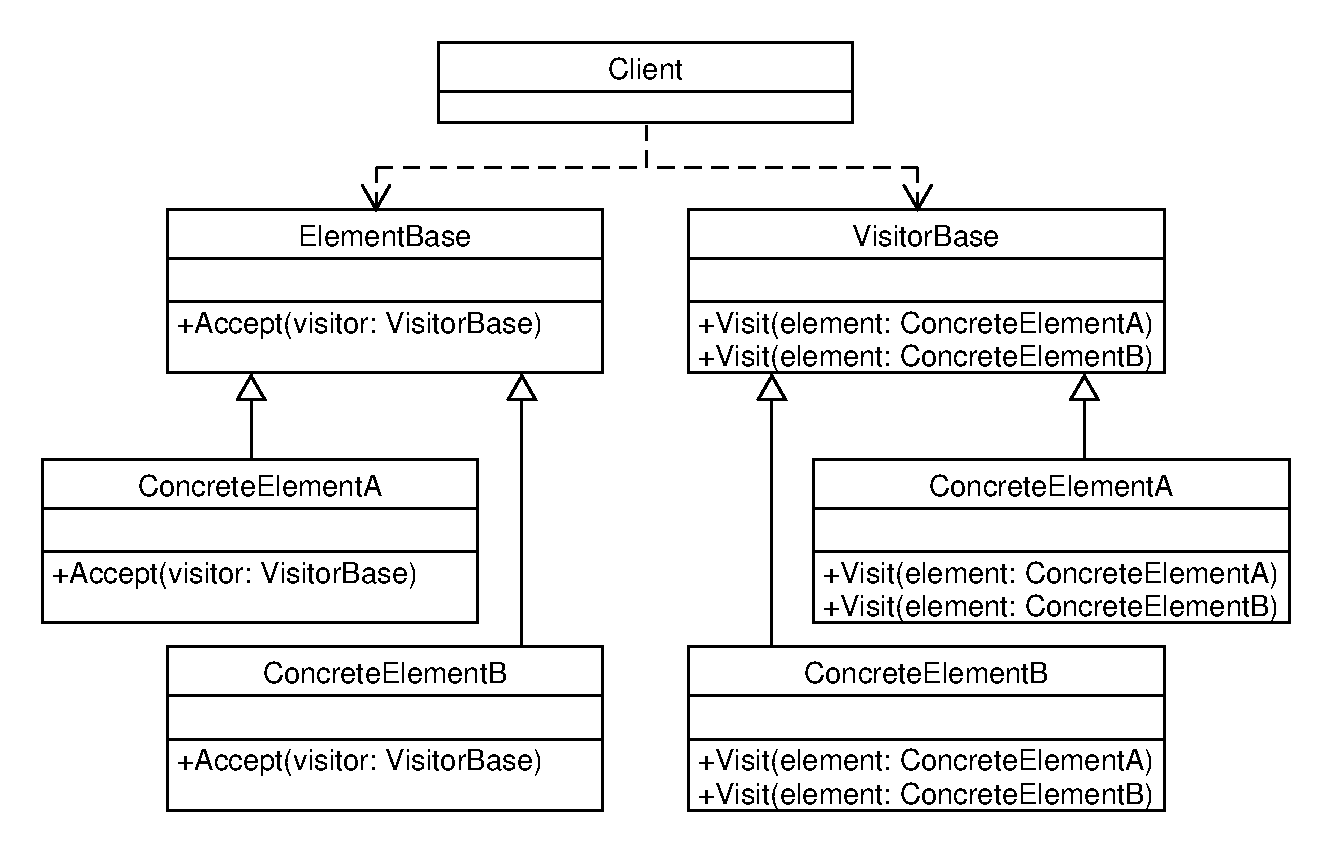
\includegraphics[width=1\textwidth]{figures/ClassDiagrams/VisitorPattern.pdf} % trim=4.85cm 15cm 0.85cm 1cm
\caption{An UML diagram for the implementation of the visitor pattern.}\label{image:visitor}
\vspace{-15pt}
\end{figure}
\todo[inline]{har vi selv lavet figuren? MP - Ja den har jeg lavet :) men der skal nok en kilde på så man kan se hvor vi har det fra, Marc found it. - Søren}

\subsection{Creating the \acrshort{ast}}\label{CreatingAst}

The goal for the \acrshort{ast} is to decrease the information in the tree.
The hidden information is then contained in fields created for the respective classes.\todo{Kan ikke finde ud af om det er lidt for groft at sige hidden information? - Søren}
Rather than having the information as fields one could also choose to have this information as children of the nodes.
This would mean that to find the information one would have to run through the children of the nodes without knowing what children it has.
The method chosen for this compiler has the information kept on the fields of a node rather than as children.
The advantage being that the information is kept together without clustering the tree and increasing the readability of the compiler.
All the nodes of the \acrshort{ast} have been designed with this in mind.
For example on figure \myref{image:ASTDecl} a class structure can be seen, which consists of all the classes needed to express a declaration from the \acrshort{cfg} on the tree.
A declaration could be \texttt{int a = 5;}.

\begin{figure}[!ht]
\centering
 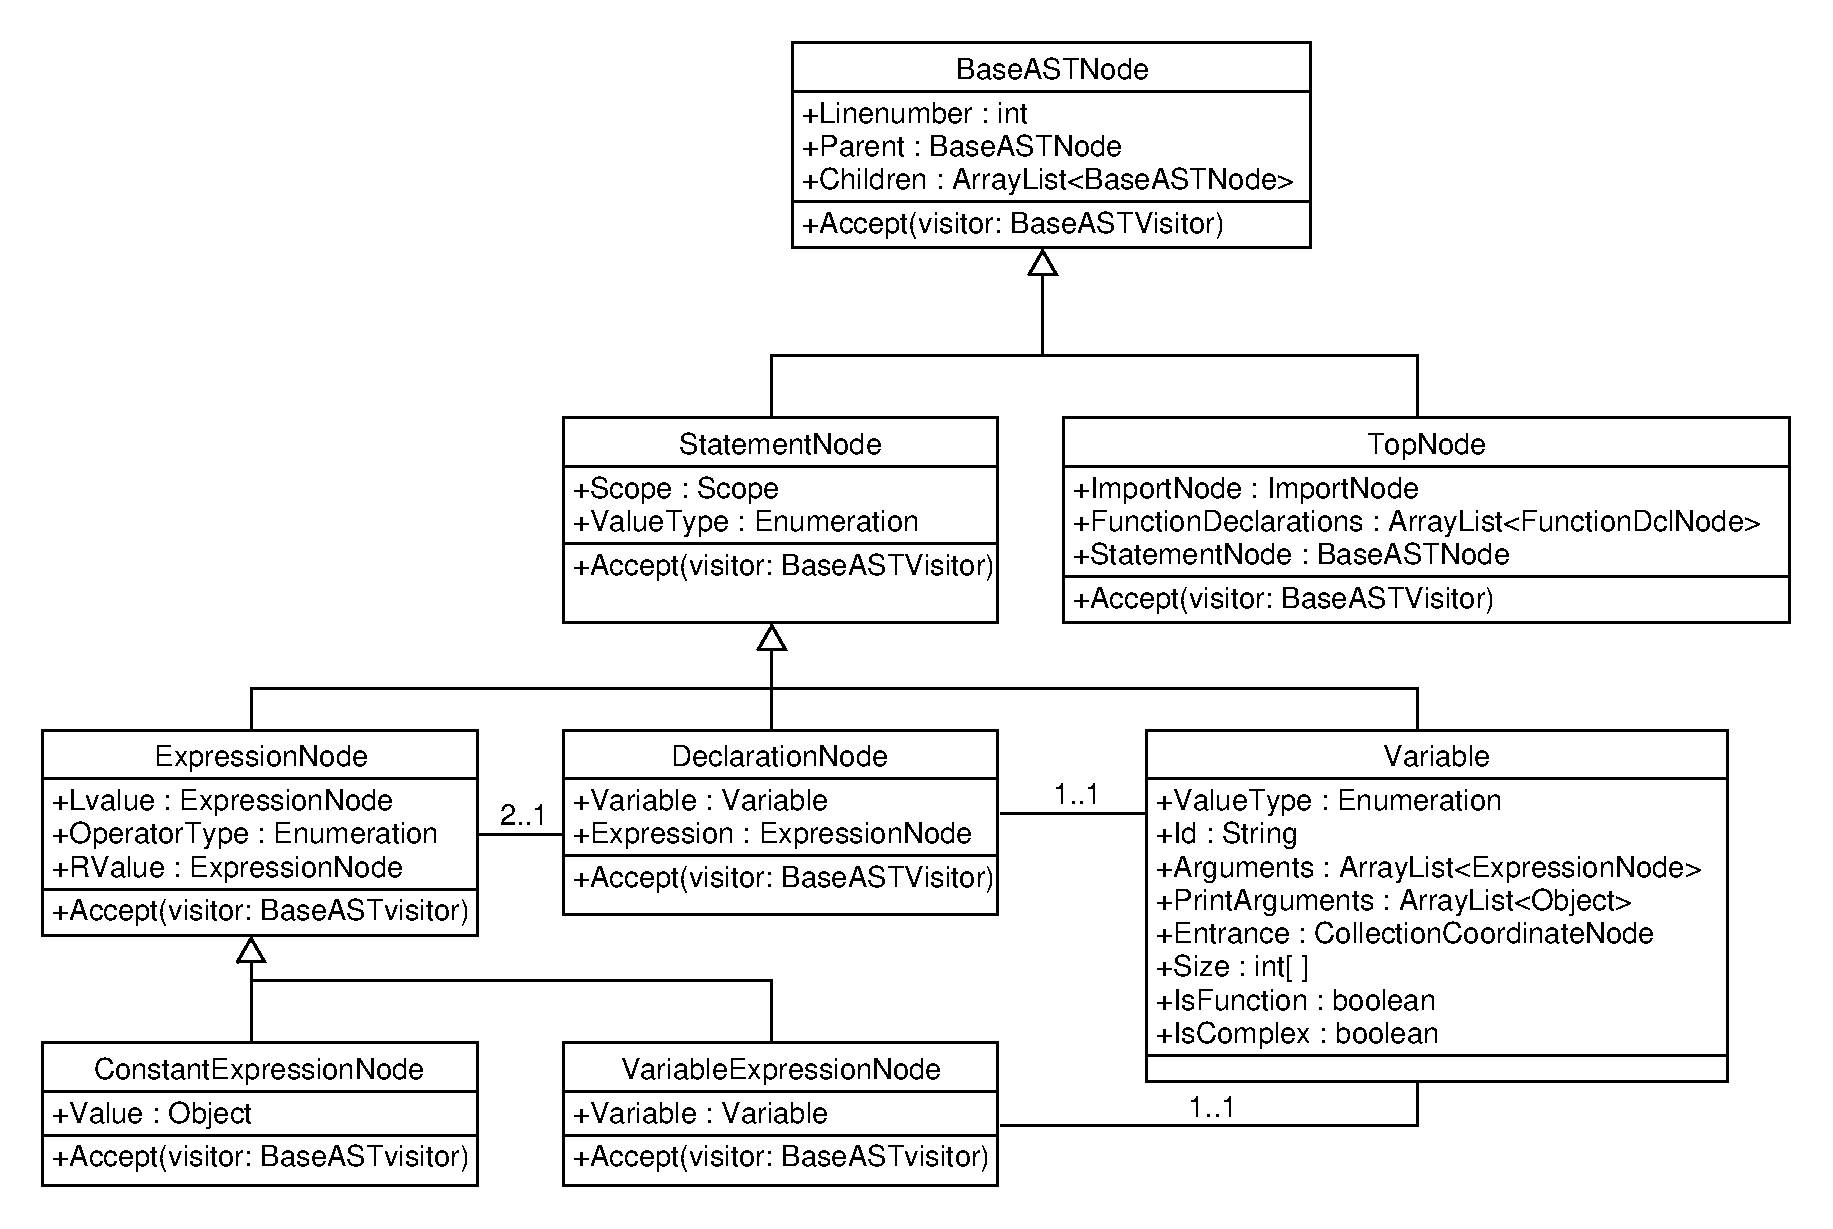
\includegraphics[width=1\textwidth]{figures/ClassDiagrams/ASTDeclarationNodeMoreInfo.pdf} % trim=4.85cm 15cm 0.85cm 1cm
\caption{A UML class diagram of the classes used for a DeclarationNode on the \acrshort{ast}.}\label{image:ASTDecl}
\vspace{-15pt}
\end{figure}

The \texttt{Variable} class contains a lot of different information which is used depending on which class a given instance of \texttt{Variable} is connected to.
If \texttt{Variable} is connected to a \texttt{VariableExpressionNode}, the only fields used on the variable class is ValueType and Id, while the booleans IsFunction and IsComplex are set to false.
In the example \texttt{int a = 5;} the tree structure looks like the AST on \myref{image:AST}.
When the right hand side of an assignment or declaration is a function, an example being \texttt{int a = foo(5);} the fields used on \texttt{Variable} differs from the previous example and instead becomes Id, ValueType, arguments, and the boolean IsFunction is now set to true.
The print argument field is used when a function call to \texttt{print()} is made. 
Entrance, Size and IsComplex are used when dealing with the complex data types, vectors and matrices.
\texttt{TopNode} sets the structure of a \gls{gamble} program as described in \myref{subsec:Struc}.
The full class diagram can be seen in \myref{ASTNodes}.

The classes have made it more intuitive to perform a traversal of the tree based upon the names of the fields on the classes.
E.g. the \texttt{ForLoopNode} has fields named \texttt{Body}, \texttt{Initialize}, \texttt{Update}, and \texttt{Conditional}, these names have meaning instead of just being children on the node which will increases the readability of the compiler.

The syntax analysis phase returns the \acrshort{ast} so it can be used in the next phase, the contextual analysis. 
The design of the phase and the call from main can be seen on \myref{fig:syntaxphase}.\todo{call from main kunne thomas ikke lide. MP - Tror det var fordi han ikke havde set figuren i compiler overview som viser alle kaldene fra main, og dermed var han forvirret over det ? Men ved det self ikke, synes bare ikke det gør noget når man også har set den figur. - Søren}
As can be seen the \texttt{GenerateASTVisitor} makes use of the classes shown in \myref{ASTNodes}.

\begin{figure}[ht]
  \centering
    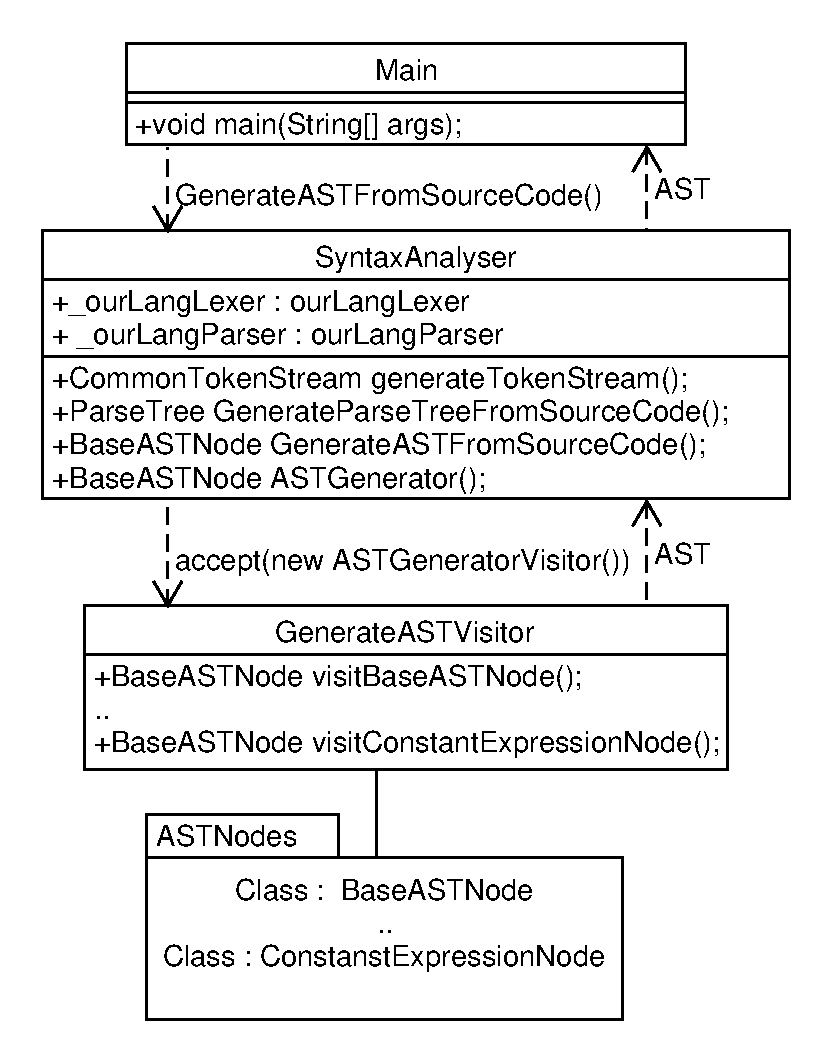
\includegraphics[width=0.48\textwidth]{figures/ClassDiagrams/SyntaxAnalyser.pdf}
  \caption{The function calls and returns in the Syntax Analysis phase.}
  \label{fig:syntaxphase}\todo{Skal vi vise at generateParseTreeFromSourceCode kaldes af ASTFromSourceCode eller noget ? - Søren}
\end{figure}
\subsection*{Abstract Syntax Tree}
\todo{to be written}
\section{Implementation}
\todo{Make this part}

\chapter{Contextual Analysis}
\section{Contextual Analysis}
\info[inline]{meta for this, phases are done in their own subsection files}
\section{Symbol Table}
In a compiler it is useful to store information about the identifiers, variables and functions in a data structure. 
This information can be useful for scope checking and type checking.

There are two common ways of implementing a Symbol Table; either you have one table which contains every identifier or you have a Symbol table for each scope. 
If constrained by memory, having a single symbol table can be beneficial, however having multiple symbol tables can simplify the code at a memory cost. 

In \gls{gamble} there exists scopes, and for each of these scopes there is a corresponding symbol table. 
Scopes inherit from each other so a scope can enclose another. 
The outermost scope, the global scope, is where functions are declared; every scope is either directly enclosed by this scope or recursively.
This means that every function can be called from anywhere within the source code - including within its' own function declarations; allowing for recursive functions. 
  

\info[inline]{Flyttes til implementationsafsnit $\downarrow$ }
In \gls{gamble} the class \texttt{SymbolTable} represents the symbol table.
The core constituent of this class is the ArrayList of the Scope class, called allScopes, meaning that every scope is stored in this ArrayList.
Every scope contains Map of Symbols and strings as keys, and information about the scope such what scope it is enclosed by. 
The key represents the name of the symbol, and must be unique to the scope and not found in an enclosing scope, as this could cause an ambiguity to arise. 
A symbol is either a variable or a function, in the class Symbol its data type, name and scope is stored. 


\section{Scope Checking}
\todo{Meta}
\subsection*{Design}
In \myref{subsec:Scope} the scope of identifiers, variables and functions, are defined for \gls{gamble}.
A variable is in scope from its declaration until the end of the block it is declared in.
An inner scope inherits the identifiers declared in the outer scopes. 

In the contextual analysis part of the compiler it is important to verify that each variable and function used are in scope, and it should produce a useful error message.
The error message should indicate which identifier is not in scope, and on what line this identifier is used wrongly.

To check this all references to identifiers must be checked to see if they match an identifier in the symbol table of the current scope, and recursively the scope which encloses it. 
Furthermore it is important that any usage of an identifier only exists after its declaration.
In the compiler for this project, the symbol table is filled while the compiler is also performing the scope checking.
This is because it reduces the amount of traversals through the tree, and scope checking and filling the symbol table is also similair in concept, e.g. a declaration creates an entry in the symbol table, while expressions simply make lookups in this table.

The scope checker produces two errors: redeclaration errors and undeclared errors.
A redeclaration error is produced when an attempt to declare a variable while it is already declarared in scope is made.
An undeclared error is produced when an attempt to use a variable which is not declared in the current scope or any enclosing scopes is made. 
Examples are shown in \myref{lst:scopeErrors}.

\begin{lstlisting}[caption=Examples of scope errors in \gls{gamble}, numbers=none,frame=tlrb,label={lst:scopeErrors}]
/* [...] */
int a = 1;
float a = 2.2;   /* Redeclaration error */
int a = 2;       /* Redeclaration error */ 

b = 2;           /* Undeclared error */   
int b = 0;
b = foo();       /* Redeclaration error and undeclared error */ 
/* [...] */
\end{lstlisting}

\subsection*{Implementation}
In the \gls{gamble} compiler, the class \texttt{SymbolTable} represents a collection of scopes.
The core constituent of this class is the ArrayList of the \texttt{Scope} class, called \texttt{allScopes}, meaning that every scope is stored in this ArrayList.
Every scope contains a hashed map with \texttt{Symbol}s as values and strings as keys.
Furthermore all scopes contain information about the particular scope such as enclosing scope and a unique id. 
The key in the hashed maps represents the name of the symbol, and must be unique to the scope and not found in an enclosing scope, as this could cause an ambiguity to arise.
This ambiguity is not allowed in \gls{gamble} and therefore generates a redeclaration error.
To determine wether or not a declaration is a redeclaration, the compiler looks up the name of the variable in the \texttt{symbolMap} of the current scope.
If no entry is found, the search continues in the \texttt{symbolMap} of the enclosing scope and outwards.
The same lookup process is executed when a variable is used e.g in a expression or assignment.
Hereby all enclosing scopes are checked for the declaration of the variable; making redeclaration of variables in scope, and usage of undeclared variables impossible in \gls{gamble}.
A symbol is an encapsulation of a variable and relevant peripheral data.
The peripheral data consists of a boolean, used for checking is a declared variable is used, and an integer with the line number if the declaration of the variable.
The boolean describing if a declared variable is used, is set to true, if the previously described lookup process for a variable in use, finds a declared variable from the unique id (the name if the variable).
This boolean also makes it possible for the \gls{gamble} compiler to find unused variables and then prompt the user with a relevant warning.

In order for all of the above to be implemented an instance of the \texttt{SymbolTable} class is passed via the constructor, to a visitor which traverses the \acrfull{ast}.
This visitor, the \texttt{SymbolTableFillVisitor} then fill the referenced \texttt{symbolTable} with scopes and their symbols.
Every time the visitor meets the start of a new scope e.g. the block of statements within a loop construct.
A new instance of the \texttt{Scope} class is pushed to the \texttt{scopeStack}, hereby making it possible to fill the relevant scope when the block of statements is visited.
At the end of a scope the top element on the \texttt{scopeStack} is popped off, and as a consequence of this the top of the \texttt{scopeStack} is back to the enclosing scope.

\section{Type Checking}
\subsection*{Design}
The second important part of the contextual analysis phase for the compiler is the type checking, which enforces the type system of \gls{gamble}.
As \gls{gamble} is statically typed it is necessary to check if all references to identifiers and constant values fit into the context they exist in. 
Since implicit conversion between floating point and integer types is not a part of \gls{gamble} an error must be issued everywhere they are used wrongly. 
It is however possible to implicitly convert between integer and floating point types internally e.g. from int16 to int64, as long as the destination variable is of a larger bit-width.
This is also the case for complex datatypes, matrices and vectors, e.g. from \texttt{matrix<float>} to \texttt{matrix<float64>}. 

The symbol table is used as a reference for which type the variable is, and therefore the type checking happens after the symbol table has been filled, hence after scope checking is completed. 
Type checking is done in many parts of the code, one or more times for each line is common. 
For every operator it must be checked if its types match and if it results in an assignment if that also matches.
Every function call must match the formal parameters of the function. 

The errors produced by the type checker are: Argument errors and type mismatch errors.
An argument error indicates that the number of arguments in the function declaration does not match the number of arguments provided in the function call.
A type mismatch error is caused by a value or identifier not being compatible (type safe) with the function parameters, operator used etc.
Examples are shown in \myref{lst:typeErrors}.

\begin{lstlisting}[caption=Examples of type errors in \gls{gamble},numbers=none,frame=tlrb,label={lst:typeErrors}]
/* [...] */
int a = 1 + 2;      /* Valid */
float b = 2.2 + 1;  /* Type mismatch error */
float c = 2;        /* Type mismatch error */

a = 2.2;            /* Type mismatch error */
b = foo(1);         /* Argument error (Takes more or fewer arguments) */ 
/* [...] */
\end{lstlisting}

\subsection*{Implementation}
The type checker is called right after the symbol table has been filled by the \texttt{SymbolTableFillVisitor}.
Since \gls{gamble} is static typed, the type checker is implemented under the contextual analysis phase of the compiler, in contrast to a dynamically typed language, such as Python or R, which is checked at runtime. \todo{er dette nødvendigt. MP}
\gls{gamble} validates the size of matrices and vectors match for certain operations as addition and multiplication E.g., as well as if they are out of bounds. 
This is to make it easier for the programmers using \gls{gamble} at a cost of speed. 
To implement type checking in the \gls{gamble} compiler a visitor is used during the contextual analysis.
The class \texttt{ASTTypeCheckVisitor} visit every relevant node in the \acrshort{ast} to check for type errors.
The class collects a list of every type error it finds, these errors is then presented to the user, when a compilation fails.
Errors and error handling are further described in \myref{subsec:DesignErrorHandling}.
The class \texttt{ASTTypeCheckVisitor} overrides the visitor calls from the \texttt{baseASTVisitor} class.
The visitor does this in multiple places in the \acrshort{ast} and the visitor uses a class \texttt{TypeChecker}, which through method calls on the variables in the nodes.
\texttt{TypeChecker} contains a method, \texttt{CombineValueTypes} which takes two values and checks if they are type compatible.
\texttt{ASTTypeCheckVisitor} visits nodes which contains either one or more variables meaning that there can be errors which should be found. 
An example of this is seen in \myref{lst:typecheck1} where the method \texttt{VisitExpressionNode}
 is shown.
The method visits an \texttt{ExpressionNode} and calls \texttt{CombineValueTypes} with the nodes left and right values if there are any available else it send \texttt{null} as the input value.
The method visits an \texttt{ExpressionNode} and uses the the \texttt{TypeChecker}s \texttt{CombineValueTypes} method, the method checks the types of the children of the \texttt{ExpressionNode} and if they fits the operator then it returns the type of the expression. 
The method returns a variable of the type returned \texttt{ValueType} and string which is printed if the visit finds type errors.

\begin{lstlisting}[caption=The VisitExprressionNode method in the ASTTypeChecker class,numbers=none,frame=tlrb,label={lst:typecheck1}]
public Variable VisitExpressionNode(ExpressionNode node) {
    ValueType valueType = TypeChecker.CombineValueTypes(
            node.getLValue() != null ? visit(node.getLValue()) : null,
            node.getRValue() != null ? visit(node.getRValue()) : null,
            errors,
            node.getLineNumber()
    );
    node.setValueType(valueType);

    return new Variable(valueType, "Expr:<" + node.toString() + ">");
}
\end{lstlisting}

After the type checker have checked every expression in the source code, the compiler scans for unused variables and thereafter prints all these as warnings. 

%Phase3
\chapter{Code Generation}
Code generation is the phase in which the object code is generated, the process and considerations this entails are covered in this chapter.
Object code is the output of the compiler.
Once the source code has passed through syntax analysis and contextual analysis without errors it has been validated and the compiler can proceed with generating the object code.
In the case of this compiler the object code is OpenCL C, as a result one or more compilers beyond this one are required to eventually end up with machine code that can be executed.\todo{more compilers? - e.g. vi bruger vores egen og gcc - Marc}
The object code is OpenCL C this means that tasks such as instruction selection and scheduling as well as register allocation will be handled by the compiler which will compile the OpenCL C code rather than \gls{gamble}.\todo{Håndterer compileren scheduling ????? - Søren - Instruction scheduling var en af de nævnte ting fra SPO kurset som man på lavniveau håndtere ja - Marc .. instruction scheduling er jo hvilken rækkefølge en given sekvens af instruktioner udføres i, ikke hvilken process har adgang til CPUen på et givent tidspunkt. -- Troels}
Furthermore in the code generation phase optimisation of the object code also takes place, for \gls{gamble} this means to create object code which is quickly executed and utilises the \acrshort{gpu} for calculation that benefit from its use.\todo{er det ok at bruge optimisation her, vi code gen'er jo bare, det er jo ikke rigtig en optimering. ? :) - Søren - Men området er referet til som optimisation, det er også derfor der efter står hvad betydningen af optimisation er for gamble - Marc }
A state diagram showing the sub-phases of the code generation can be seen in \myref{fig:flowCodegen}.

\vspace{10pt}
\begin{figure}[h]
    \centering
    \begin{tikzpicture}[node distance = 3cm, auto]
        %\node (invi1) [invi, draw=none] {};
        %\node (ast) [lille, below=-0.35cm of invi1] {Abstract Syntax Tree};
        %\node (symboltable) [lille, minimum width=6.75cm, minimum height=2.4cm, right=2cm of invi1, fill=blue!10, label={[xshift=0cm, yshift=-1cm]Symbol Table}] {};
        %\node (scope) [lille, right=1.1cm of ast] {Scopechecker};
        %\node (type) [lille, right=0.7cm of scope] {Typechecker};
        %\node (dast) [lille, right=1.1cm of type] {Decorated Abstact Syntax Tree};

        %\node (error) [cloud, below=1cm of symboltable] {Error report};

        %\draw [arrow] (ast) -- (scope);
        %\draw [arrow] (scope) -- (type);
        %\draw [arrow] (type) -- (dast);
        %\draw [arrow,dashed] (scope) -- (error);
        %\draw [arrow,dashed] (type) -- (error);
        %\draw [arrow,dashed] (symboltable) -- (error);

        \node (dast) [lille, align=left] {Contextual \\Analysis Phase};
        \node (cgv) [lille, right=0.7cm of dast, align=left] {Code Generation \\Visitor};
        \node (copy) [lille, right=0.7cm of cgv] {Output \gls{opencl} C code};
        \node (error) [invi, draw=none, minimum width=2cm, right=1cm of copy, label={[xshift=40pt, yshift=-17pt]Finished Compilation}] {};

        \draw[black,fill=black, above=1cm of parser] (10.9,0) circle (1ex);
        \draw[black, above=1cm of parser] (10.9,0) circle (1.3ex); 

        \draw [arrow] (dast) -- (cgv);
        \draw [arrow] (cgv) -- (copy);
        \draw [arrow] (copy) -- (error);
    \end{tikzpicture}
    \caption{State diagram showing the modules of the code generation. } 
    \label{fig:flowCodegen}
\end{figure}
\vspace{-20pt}


\info[inline]{next chapters are : Test of language, Conclusion, and Perspektivaaation(top kek)}
